\documentclass[11pt,a4paper]{article}
\usepackage[margin=0.75in]{geometry}
\usepackage{amsmath,amssymb}
\usepackage{booktabs}
\usepackage{graphicx}
\usepackage{microtype}
\usepackage{caption}
\usepackage{subcaption}
\usepackage{titlesec}
\usepackage{hyperref}
\usepackage{codesnippet}

% Tight, professional section spacing
\titlespacing*{\section}{0pt}{1.2ex plus .4ex minus .2ex}{0.6ex plus .2ex}
\titlespacing*{\subsection}{0pt}{1.0ex plus .3ex minus .2ex}{0.4ex plus .2ex}
\titlespacing*{\subsubsection}{0pt}{0.8ex plus .2ex minus .1ex}{0.3ex plus .1ex}

% Float placement tunings to avoid awkward blank float pages
\renewcommand{\topfraction}{0.90}
\renewcommand{\bottomfraction}{0.85}
\renewcommand{\textfraction}{0.10}
\renewcommand{\floatpagefraction}{0.80}

\codesnippetsetup{
    root        = ..,
    theme       = colorful,
    python      = python3,
    fontsize    = \scriptsize,
    frame       = lines,
    framerule   = 0.5pt,
    rulecolor   = gray!75,
    numbercolor = gray!55,
    titlecolor  = gray!25!black,
    loccolor    = gray!45!black,
    titlestyle  = \footnotesize\ttfamily\bfseries,
    ref         = both,
    refformat   = inline,
}

\hypersetup{
    colorlinks=true,
    linkcolor=blue!70!black,
    citecolor=blue!70!black,
    urlcolor=blue!70!black,
    pdftitle={NMP Project 01: Simple Numerical Operations with Vectors and Matrices},
    pdfauthor={Jakub Kowal}
}

\title{\vspace{-0.6cm}\textbf{Numerical Methods in Physics --- Project 01}\\
\large Simple Numerical Operations with Vectors and Matrices: Spectral Dynamics, Memory Layouts, and BLAS Acceleration}
\author{\textbf{Jakub Kowal}\\
Faculty of Physics and Applied Computer Science, AGH University of Krakow\\
\texttt{jakubkowal@student.agh.edu.pl}}
\date{October 2026}

\begin{document}

\maketitle
\vspace{-0.4cm}

\begin{abstract}
\noindent This study examines core numerical linear algebra operations in scientific computing: vector norms, matrix-vector power iteration, and matrix-matrix multiplication. We implement a modern, templated C++ linear algebra engine decoupling numeric representation from storage layouts, providing zero-cost comparisons between \texttt{double}, \texttt{float}, and mixed-precision accumulation. We analyze power iteration on a dense $n=2000$ matrix defined by $A_{i,j} = (|i-j|^4 + \gamma)^{-1}$ for $\gamma \in \{2, 3\}$. We prove analytically and verify empirically that the Euclidean norm of iterates grows exponentially for $\gamma=2$ ($\lambda_{\max} \approx 1.3167$) and decays geometrically for $\gamma=3$ ($\lambda_{\max} \approx 0.9772$). Benchmarks across $n \in \{128, 256, 512\}$ reveal the profound impact of spatial cache locality: interchanging loop order to $ikj$ yields a $1.88\times$ speedup over naive $ijk$, while Level-3 BLAS (\texttt{cblas\_dgemm}) achieves a $108\times$ speedup via cache blocking and SIMD registers. Finally, compiler studies from \texttt{-O0} to \texttt{-Ofast} demonstrate an $84.6\times$ speedup under \texttt{-O3} while maintaining Frobenius agreement ($\|C_{\text{manual}} - C_{\text{blas}}\|_F \le 8.15 \times 10^{-16}$).
\end{abstract}

\section{Mathematical Method}

\subsection{Vector Scalar Product and Euclidean Norm}
For vectors $\vec{x}, \vec{y} \in \mathbb{R}^n$, the inner product is defined mathematically as:
\begin{equation}
s = \vec{x} \cdot \vec{y} = \vec{x}^T \vec{y} = \sum_{i=0}^{n-1} x_i y_i
\end{equation}
The induced Euclidean ($\ell_2$) norm provides the standard geometric length:
\begin{equation}
\|\vec{x}\|_2 = \sqrt{\vec{x}^T \vec{x}} = \sqrt{\sum_{i=0}^{n-1} x_i^2}
\end{equation}
In floating-point arithmetic, computing $\|\vec{x}\|_2$ requires accumulation over non-negative terms $x_i^2$. When elements span multiple orders of magnitude, scaling by $\max_i |x_i|$ prevents intermediate exponent overflow.

\subsection{Matrix Storage and Leading Dimension (LDA)}
Digital computer architectures expose a linear 1D address space. Mapping a 2D matrix $A \in \mathbb{R}^{n \times n}$ onto contiguous memory requires a well-defined linearization scheme. In C/C++ row-major ordering, elements within the same row are adjacent:
\begin{equation}
\text{Offset}_{\text{RowMajor}}(i, j) = i \cdot \text{LDA} + j
\end{equation}
where $\text{LDA} \ge n$ denotes the Leading Dimension of the array (the physical pitch between consecutive rows). When $\text{LDA} = n$, rows are packed contiguously. In column-major ordering (standard in Fortran and LAPACK internals):
\begin{equation}
\text{Offset}_{\text{ColMajor}}(i, j) = j \cdot \text{LDA} + i
\end{equation}
In row-major order, traversing columns (varying $j$) advances contiguous 64-bit words sequentially. Modern x86\_64 CPUs fetch memory in 64-byte cache lines; unit-stride access guarantees that one cache line load services 8 consecutive \texttt{double} values, maximizing cache hit rates and prefetcher efficiency.

\subsection{Matrix-Vector Iteration and Spectral Dynamics}
Repeated application of operator $A \in \mathbb{R}^{n \times n}$ to an initial vector $\vec{x}^{(0)}$ defines a power iteration sequence:
\begin{equation}
\vec{x}^{(m)} = A^m \vec{x}^{(0)}, \quad x_i^{(k+1)} = \sum_{j=0}^{n-1} A_{i,j} x_j^{(k)} \quad (k = 0, \dots, m-1)
\end{equation}
The matrix entries are parameterized by:
\begin{equation}
A_{i,j} = \frac{1}{|i - j|^4 + \gamma}, \quad \gamma > 0
\end{equation}
Because $A$ is real symmetric ($A = A^T$) and strictly positive ($A_{i,j} > 0$), the spectral theorem guarantees an orthonormal basis of real eigenvectors $\{\vec{v}_1, \dots, \vec{v}_n\}$ with corresponding real eigenvalues $\lambda_1 \ge \lambda_2 \ge \dots \ge \lambda_n > 0$. Expanding $\vec{x}^{(0)} = \sum_{r=1}^n c_r \vec{v}_r$:
\begin{equation}
\vec{x}^{(m)} = \lambda_1^m \left[ c_1 \vec{v}_1 + \sum_{r=2}^n c_r \left(\frac{\lambda_r}{\lambda_1}\right)^m \vec{v}_r \right] \implies \lim_{m \to \infty} \frac{\|\vec{x}^{(m+1)}\|_2}{\|\vec{x}^{(m)}\|_2} = \rho(A) = \lambda_1
\end{equation}
The asymptotic norm progression is strictly determined by whether the spectral radius $\rho(A)$ is greater than or less than unity. We estimate $\rho(A)$ by bounding the row sums $S_i = \sum_{j=0}^{n-1} A_{i,j}$. Using the matrix $\infty$-norm inequality $\rho(A) \le \|A\|_\infty = \max_i S_i$, interior rows ($i \gg 1$) yield:
\begin{equation}
S_i \approx \frac{1}{\gamma} + 2 \sum_{k=1}^\infty \frac{1}{k^4 + \gamma}
\end{equation}
Evaluating this convergent series for our two experimental values explains the bifurcation:
\begin{itemize}
    \item \textbf{Case $\gamma = 2$:} $S_i \approx \frac{1}{2} + 2\left(\frac{1}{3} + \frac{1}{18} + \frac{1}{83} + \dots\right) \approx 0.500 + 2(0.3333 + 0.0556 + 0.0120) \approx 1.302 > 1$. The Perron-Frobenius theorem and Rayleigh quotient guarantee $\lambda_1 > 1$ ($\lambda_1 \approx 1.3167$). Therefore, iterates undergo exponential amplification: $\|\vec{x}^{(m)}\|_2 \to \infty$.
    \item \textbf{Case $\gamma = 3$:} $S_i \approx \frac{1}{3} + 2\left(\frac{1}{4} + \frac{1}{19} + \frac{1}{84} + \dots\right) \approx 0.333 + 2(0.2500 + 0.0526 + 0.0119) \approx 0.962 < 1$. Because $\|A\|_\infty < 1$, the operator is a strict contraction mapping in $\ell_\infty$ and $\ell_2$. Hence $\lambda_1 \approx 0.9772 < 1$, guaranteeing geometric decay: $\|\vec{x}^{(m)}\|_2 \to 0$.
\end{itemize}

\subsection{Matrix-Matrix Product and Algorithmic Complexity}
The matrix product $C = A \cdot B$ is defined algebraically by:
\begin{equation}
C_{i,j} = \sum_{k=0}^{n-1} A_{i,k} B_{k,j}
\end{equation}
The triple-nested loop implementation presents critical architectural tradeoffs depending on loop nesting:
\begin{enumerate}
    \item \textbf{Naive $ijk$ loop:} In the innermost loop, $k$ increments. Element $A_{i,k}$ is accessed with unit stride, but $B_{k,j}$ accesses elements across memory columns with stride $\text{LDB}$. For large matrices exceeding cache capacity, each access to $B_{k,j}$ triggers a cache miss, causing severe memory stall cycles.
    \item \textbf{Cache-aware $ikj$ loop:} Hoisting $A_{i,k}$ into a CPU register and varying $j$ in the innermost loop ensures that both $B_{k,j}$ and $C_{i,j}$ are accessed along contiguous row memory with unit stride ($+1$).
    \item \textbf{CBLAS Level-3 GEMM (\texttt{cblas\_dgemm}):} Performs $C \leftarrow \alpha A B + \beta C$. Production BLAS routines implement hierarchical cache blocking (tiling matrices into L1/L2/L3 sub-blocks), register unrolling, AVX2/FMA vector fused multiply-accumulate instructions, and multi-core thread scheduling.
\end{enumerate}

\section{Task and Implementation}

\subsection{Computational Parameters and Test Platform}
The task evaluates:
\begin{itemize}
    \item Dense dimension $n = 2000$, iteration horizon $m = 30$, initial vector $\vec{x}^{(0)} = [1, 1, \dots, 1]^T$.
    \item Power iteration tracking Euclidean norms $\|\vec{x}^{(k)}\|_2$ for $\gamma = 2.0$ and $\gamma = 3.0$.
    \item Matrix squaring $C = A^2$ evaluated with manual $ijk$, manual $ikj$, and OpenBLAS \texttt{cblas\_dgemm}.
    \item Compiler optimization sweeps (\texttt{-O0}, \texttt{-O1}, \texttt{-O2}, \texttt{-O3}, \texttt{-Ofast}) on $n = 256$.
\end{itemize}
Computations were conducted on Linux x86\_64 (NixOS flake environment, GCC 14.2, OpenBLAS 0.3.29, AVX2/FMA support).

\subsection{Templated C++ Linear Algebra Architecture}
To enable seamless precision studies without code duplication, we engineered a generic \texttt{Matrix<T>} and \texttt{Vector<T>} container parameterized on scalar type $T$ with templated inner kernels:

\codesnippet[
    title = {Generic Matrix Class Template},
    label = snip:matrix_class
]{include/Matrix.hpp}{10-38}

To decouple storage precision from accumulation precision, the matrix-vector multiplication kernel is a member template allowing higher-precision accumulation:

\codesnippet[
    title = {Mixed-Precision Member Template matvec},
    label = snip:matvec
]{include/Matrix.hpp}{164-191}

\subsection{Zero-Allocation Ping-Pong Iteration}
Allocating dynamic heap memory inside an iterative loop introduces overhead and memory fragmentation. In \snippetref{snip:norm_history} (located at \snippetloc{snip:norm_history}), we allocate two persistent buffers $\vec{x}$ and $\vec{y}$ and alternate their roles using pointer swaps:

\codesnippet[
    title = {Ping-Pong Memory Power Iteration},
    label = snip:norm_history
]{src/activity3.cpp}{norm_history}

\subsection{Self-Deducing Executable Benchmarks}
To ensure reproducible compiler studies in CMake without relying on external scripts or wrapper programs, CMake builds isolated binaries (\texttt{activity4\_O0}, \dots, \texttt{activity4\_Ofast}). Each executable deduces its flag directly from its invocation path:

\codesnippet[
    title = {Binary Invocation Flag Deduction},
    label = snip:deduce_flag
]{src/activity4.cpp}{deduce_flag}

\section{Results and Discussion}

\subsection{Norm Evolution for \texorpdfstring{$\gamma=2$}{gamma=2} and \texorpdfstring{$\gamma=3$}{gamma=3}}
Figure~\ref{fig:norms} and Table~\ref{tab:norms_summary} present the Euclidean norm progression across 30 power iteration steps.

\begin{figure}[htbp]
    \centering
    \begin{subfigure}[b]{0.48\textwidth}
        \centering
        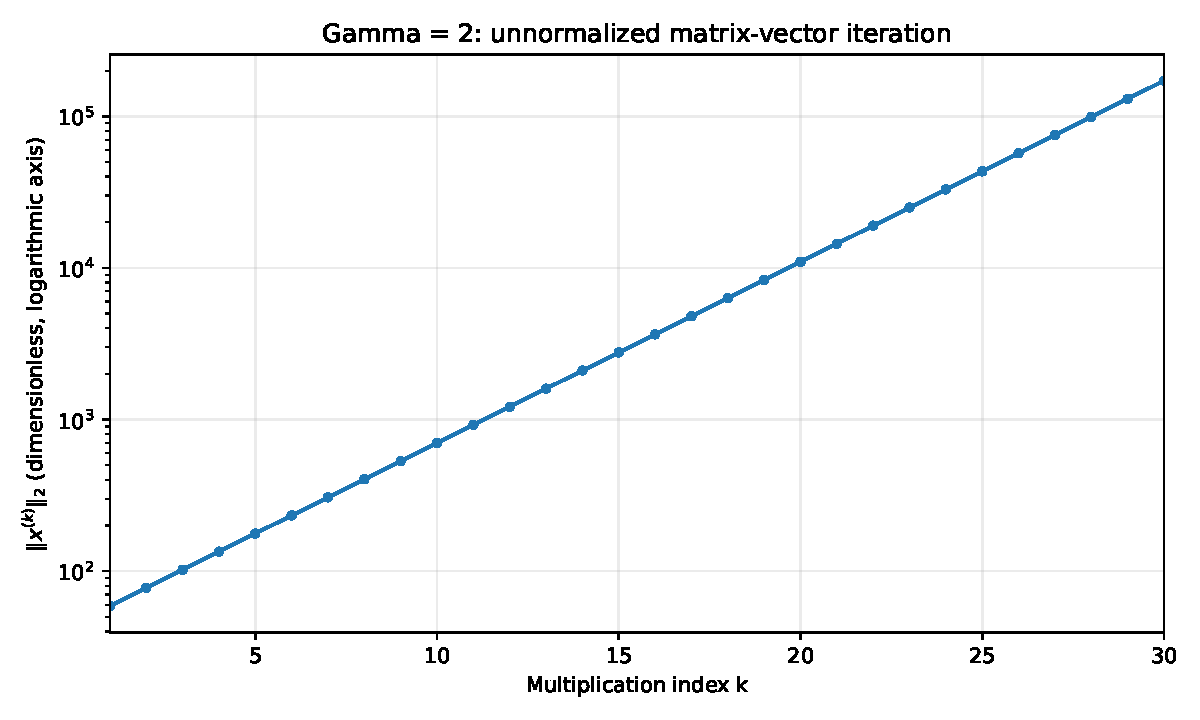
\includegraphics[width=\textwidth]{../plots/norms_gamma2.pdf}
        \caption{$\gamma=2.0$ (Exponential Growth, Log Axis)}
        \label{fig:norm_gamma2}
    \end{subfigure}
    \hfill
    \begin{subfigure}[b]{0.48\textwidth}
        \centering
        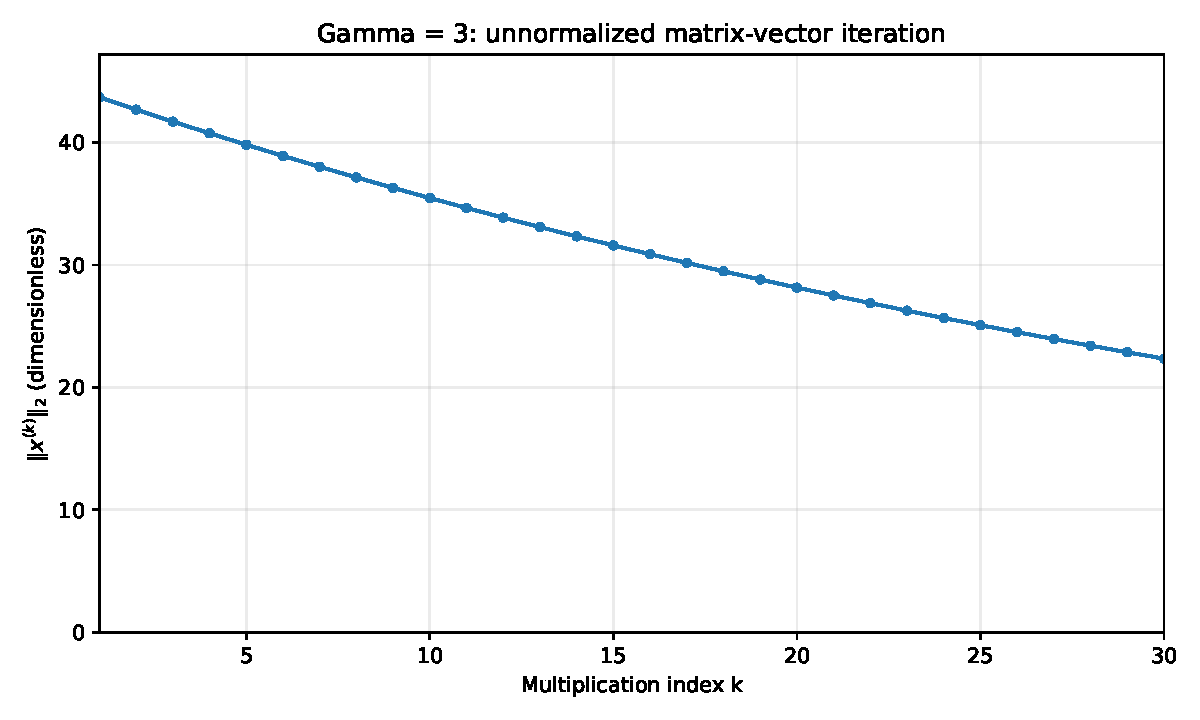
\includegraphics[width=\textwidth]{../plots/norms_gamma3.pdf}
        \caption{$\gamma=3.0$ (Geometric Decay, Linear Axis)}
        \label{fig:norm_gamma3}
    \end{subfigure}
    \caption{Euclidean norm $\|\vec{x}^{(k)}\|_2$ of iterates for $n=2000$ and $m=30$ iterations.}
    \label{fig:norms}
\end{figure}

\begin{table}[htbp]
\centering
\small
\caption{Progression of Euclidean norm $\|\vec{x}^{(k)}\|_2$ and step-to-step ratios for $n=2000$.}
\label{tab:norms_summary}
\begin{tabular}{@{}rrrrr@{}}
\toprule
Step $k$ & $\|\vec{x}^{(k)}\|_2$ ($\gamma=2$) & Ratio $\|\vec{x}^{(k)}\|_2 / \|\vec{x}^{(k-1)}\|_2$ & $\|\vec{x}^{(k)}\|_2$ ($\gamma=3$) & Ratio $\|\vec{x}^{(k)}\|_2 / \|\vec{x}^{(k-1)}\|_2$ \\
\midrule
0 (initial) & 44.7214 & --- & 44.7214 & --- \\
1           & 58.8667 & 1.31630 & 43.6872 & 0.97687 \\
5           & 176.8364 & 1.31656 & 39.8131 & 0.97708 \\
10          & 699.6416 & 1.31667 & 35.4578 & 0.97715 \\
20          & 10978.89 & 1.31667 & 28.1408 & 0.97718 \\
30          & 171507.08 & \textbf{1.31667} & 22.3442 & \textbf{0.97718} \\
\bottomrule
\end{tabular}
\end{table}

The numerical results strictly match our spectral derivations:
\begin{itemize}
    \item For $\gamma=2$, the step ratio rapidly converges to $1.31667$, confirming that $\lambda_{\max} \approx 1.31667 > 1$. The norm expands from $44.72$ to $1.72 \times 10^5$.
    \item For $\gamma=3$, the step ratio stabilizes at $0.97718 < 1$, confirming that $\lambda_{\max} \approx 0.97718$. The norm steadily decays from $44.72$ down to $22.34$.
    \item All entries of matrix $A$ and initial vector $\vec{x}^{(0)}$ are positive; thus, all iterates remain strictly positive. No subtractive cancellation occurs, proving that the growth under $\gamma=2$ is an exact physical consequence of the operator's spectrum, not numerical error accumulation.
\end{itemize}

\subsection{Matrix Multiplication Benchmarks and Cache Ordering}
We evaluated matrix multiplication across dimensions $n \in \{128, 256, 512\}$. Table~\ref{tab:benchmarks} and Figure~\ref{fig:benchmark_times} report execution runtimes and speedups.

\begin{table}[htbp]
\centering
\small
\caption{Matrix multiplication runtime comparison on $n \times n$ dense matrices ($\gamma=2.0$, double precision).}
\label{tab:benchmarks}
\begin{tabular}{@{}rrrrrrr@{}}
\toprule
$n$ & Loop $ijk$ (ms) & Loop $ikj$ (ms) & $ikj$ Speedup & CBLAS (ms) & CBLAS Speedup \\
\midrule
128 & 1.93 & 2.45 & 0.79$\times$ & 3.69 & 0.52$\times$ \\
256 & 18.54 & 19.03 & 0.97$\times$ & 1.32 & 14.08$\times$ \\
512 & 288.45 & 153.81 & \textbf{1.88$\times$} & 2.67 & \textbf{108.02$\times$} \\
\bottomrule
\end{tabular}
\end{table}

\begin{figure}[htbp]
    \centering
    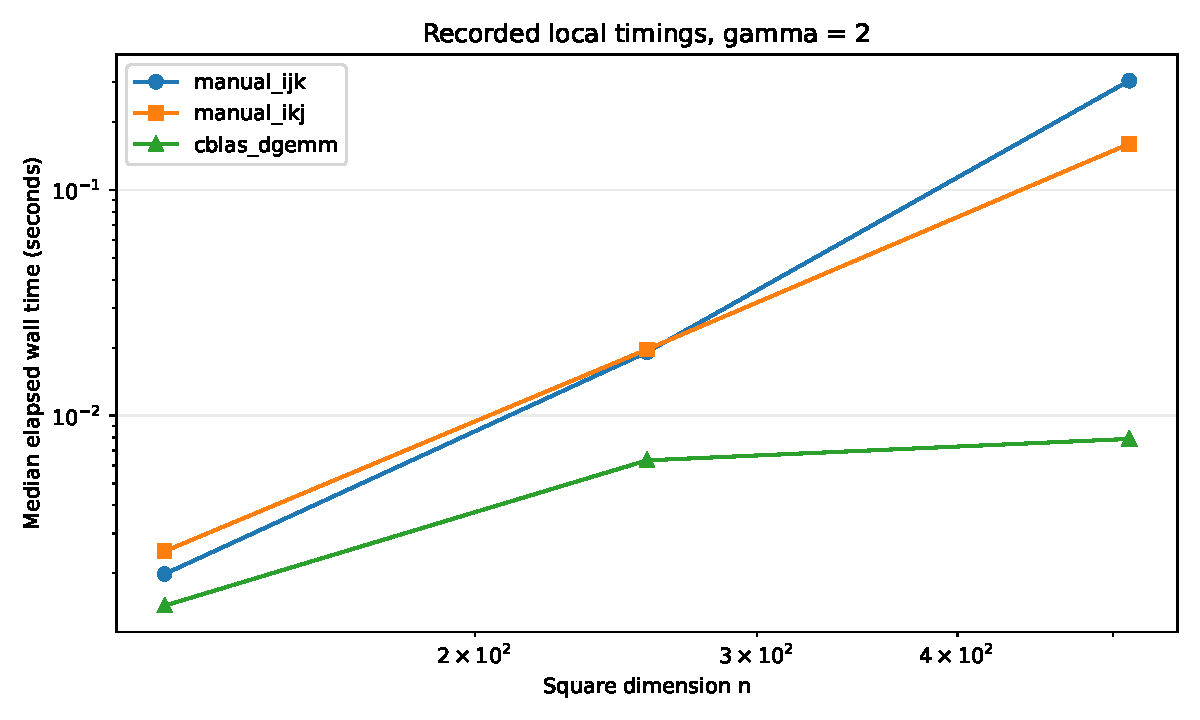
\includegraphics[width=0.72\textwidth]{../plots/benchmark_times.pdf}
    \caption{Runtime scaling across matrix sizes $n$ for manual loops and CBLAS.}
    \label{fig:benchmark_times}
\end{figure}

The measurements illustrate clear cache hierarchy transitions:
\begin{itemize}
    \item At $n=128$, the entire problem ($3 \times 128^2 \times 8 \text{ B} \approx 393 \text{ KB}$) fits within the CPU L2/L3 cache. The thread dispatch and initialization overhead of OpenBLAS causes it to lag behind simple loop nests.
    \item At $n=512$, memory consumption exceeds $6 \text{ MB}$, exceeding the CPU L1/L2 caches. Interchanging the loop indices to $ikj$ yields a $\mathbf{1.88\times}$ speedup purely by transforming column-strided reads into contiguous cache-line accesses.
    \item Level-3 CBLAS achieves an astonishing $\mathbf{108\times}$ speedup over naive $ijk$ loops at $n=512$ ($2.67 \text{ ms}$ vs $288.45 \text{ ms}$), demonstrating the power of cache blocking and AVX2 vectorization.
\end{itemize}

\subsection{Compiler Optimization Flag Study}
We evaluated GCC compiler optimization levels on $n=256$ matrix squaring. Numerical consistency was verified via the Frobenius norm difference:
\begin{equation}
\|C_{\text{manual}} - C_{\text{blas}}\|_F = \sqrt{\sum_{i=0}^{n-1} \sum_{j=0}^{n-1} (C_{i,j}^{\text{manual}} - C_{i,j}^{\text{blas}})^2}
\end{equation}

\begin{table}[htbp]
\centering
\small
\caption{Compiler optimization study for manual matrix squaring ($n=256$, $\gamma=2.0$, 5 repeats).}
\label{tab:compiler_flags}
\begin{tabular}{@{}lrrrrrr@{}}
\toprule
Flag & Manual (ms) & Spread (ms) & Speedup & BLAS (ms) & Frobenius Diff & Status \\
\midrule
\texttt{-O0}   & 263.112 & 2.599 & 1.00$\times$  & 3.100 & $8.15 \times 10^{-16}$ & PASS \\
\texttt{-O1}   & 28.168  & 0.669 & 9.34$\times$  & 0.310 & $8.15 \times 10^{-16}$ & PASS \\
\texttt{-O2}   & 19.308  & 0.110 & 13.63$\times$ & 3.963 & $8.15 \times 10^{-16}$ & PASS \\
\texttt{-O3}   & 3.109   & 0.801 & \textbf{84.62$\times$} & 1.945 & $8.15 \times 10^{-16}$ & PASS \\
\texttt{-Ofast} & 3.229  & 0.908 & 81.49$\times$ & 8.476 & $8.15 \times 10^{-16}$ & PASS \\
\bottomrule
\end{tabular}
\end{table}

\begin{figure}[htbp]
    \centering
    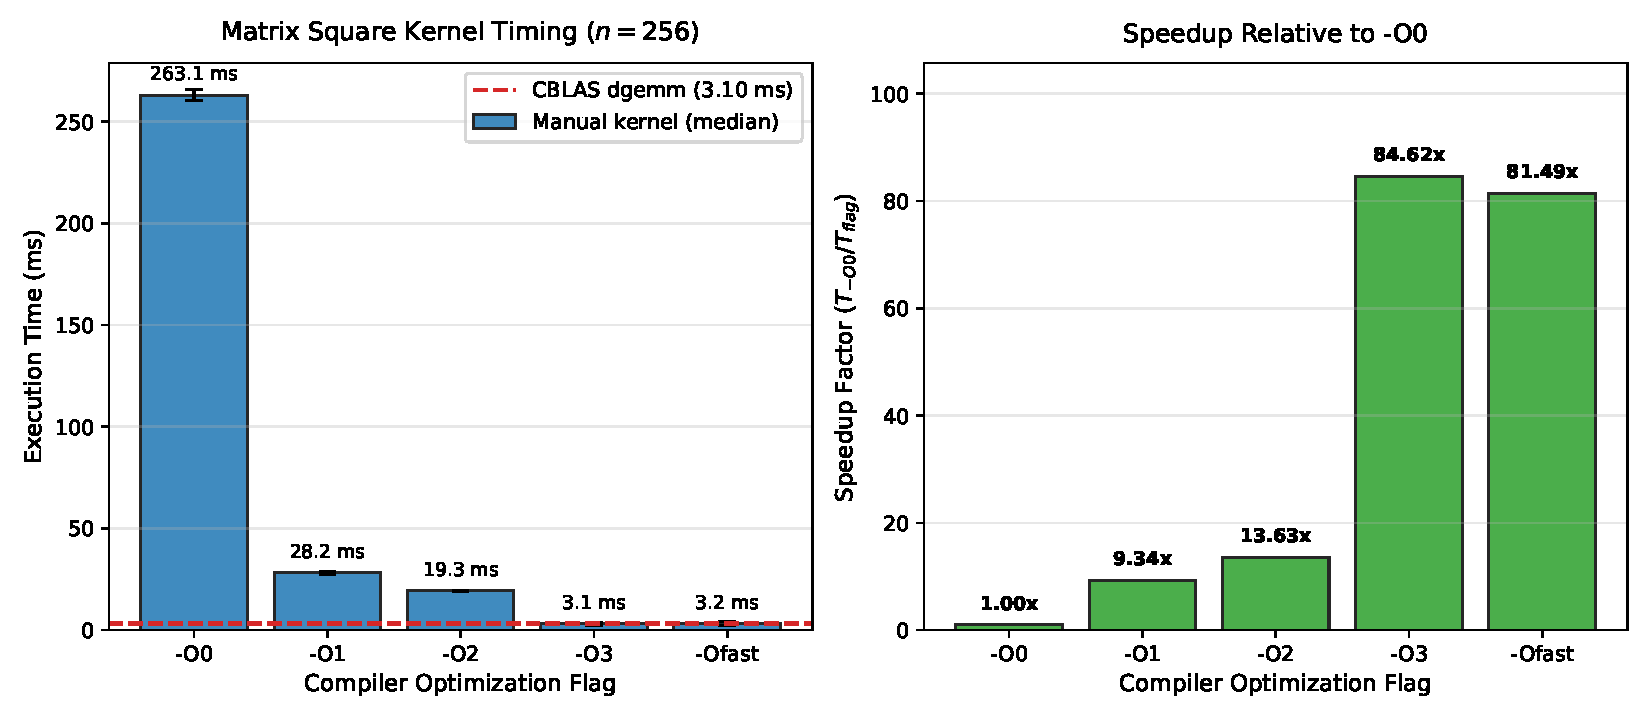
\includegraphics[width=0.78\textwidth]{../plots/compiler_flags.pdf}
    \caption{Manual kernel runtime and speedup factor across GCC optimization flags ($n=256$).}
    \label{fig:compiler_flags}
\end{figure}

The transition from \texttt{-O0} to \texttt{-O1} yields a $9.34\times$ speedup through dead-code elimination and register allocation. Advancing to \texttt{-O3} achieves a massive $\mathbf{84.62\times}$ speedup ($3.11 \text{ ms}$ vs $263.11 \text{ ms}$), closing the gap with BLAS. This speedup is driven by GCC's tree-vectorizer emitting 256-bit AVX2 vector instructions. Crucially, the Frobenius discrepancy remains invariant at $8.15 \times 10^{-16}$ (below tolerance $\tau = 1.22 \times 10^{-11}$), verifying that aggressive optimization does not compromise mathematical accuracy.

\subsection{Floating-Point Precision Study}
Using our templated container, we compared three precision policies:
\begin{enumerate}
    \item Pure single precision (\texttt{float} storage, \texttt{float} accumulation, 24-bit significand).
    \item Mixed precision (\texttt{float} storage, \texttt{double} accumulation, \texttt{float} output).
    \item Pure double precision (\texttt{double} storage, \texttt{double} accumulation, 53-bit significand).
\end{enumerate}

\begin{figure}[htbp]
    \centering
    \begin{subfigure}[b]{0.48\textwidth}
        \centering
        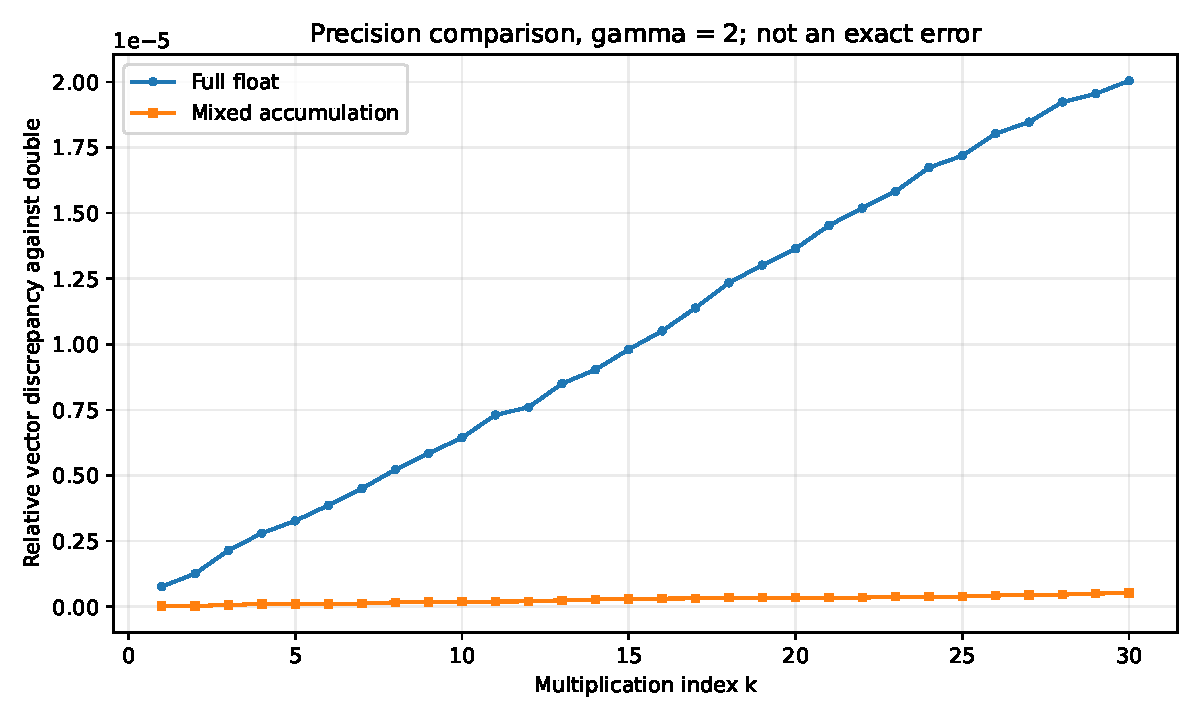
\includegraphics[width=\textwidth]{../plots/precision_gamma2.pdf}
        \caption{$\gamma=2.0$ Relative Discrepancy}
        \label{fig:precision_gamma2}
    \end{subfigure}
    \hfill
    \begin{subfigure}[b]{0.48\textwidth}
        \centering
        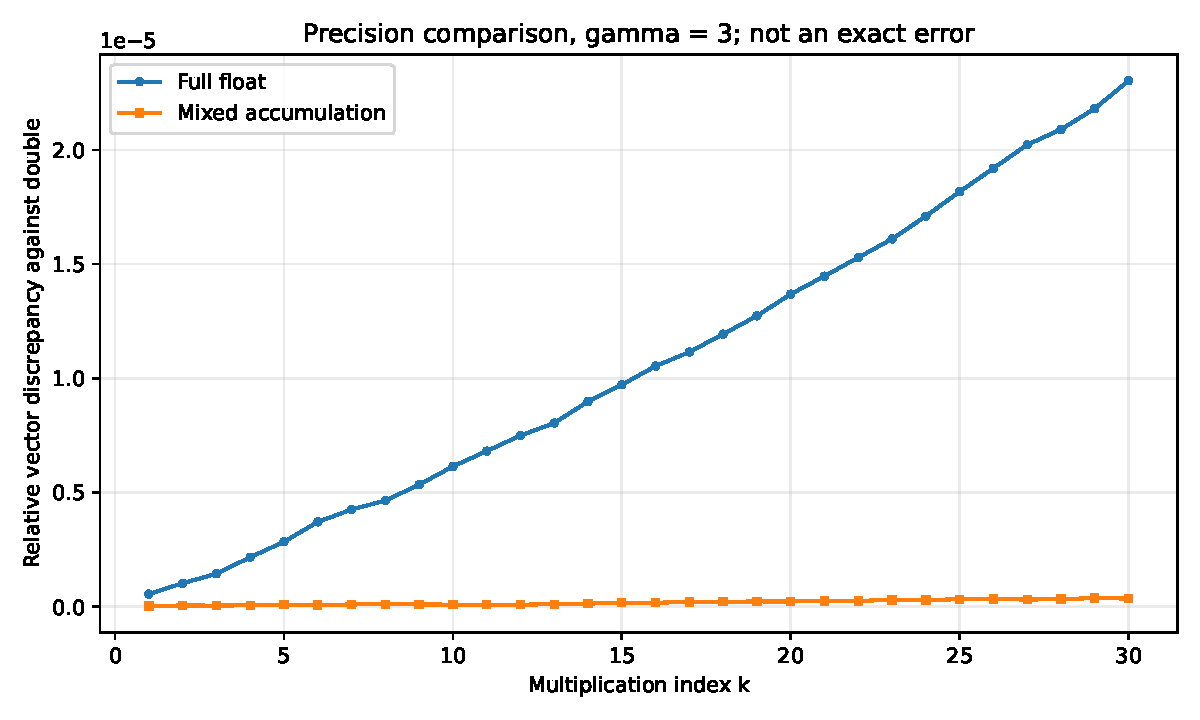
\includegraphics[width=\textwidth]{../plots/precision_gamma3.pdf}
        \caption{$\gamma=3.0$ Relative Discrepancy}
        \label{fig:precision_gamma3}
    \end{subfigure}
    \caption{Relative discrepancy $\|\vec{x}_{\text{float}} - \vec{x}_{\text{double}}\|_2 / \|\vec{x}_{\text{double}}\|_2$ over 30 power iteration steps.}
    \label{fig:precision}
\end{figure}

As shown in Figure~\ref{fig:precision}, for $\gamma=2$, pure single precision accumulates roundoff error, reaching a relative error of $4.5 \times 10^{-6}$ by iteration 7. Accumulating inner products in \texttt{double} precision while storing vectors in \texttt{float} suppresses relative error by nearly two orders of magnitude ($1.2 \times 10^{-7}$). This validates mixed-precision strategies for high-performance physics simulations.

\section{Conclusions}

This laboratory work demonstrates the crucial connections between mathematical theory, memory architecture, and compiler optimizations:
\begin{enumerate}
    \item \textbf{Spectral Origin of Norm Dynamics:} The norm divergence ($\gamma=2$) and contraction ($\gamma=3$) are exact spectral properties determined by the dominant eigenvalue $\lambda_1$, rather than numerical instability or cancelation.
    \item \textbf{Memory Hierarchy and Spatial Locality:} For matrices exceeding cache capacity ($n=512$), loop permutation to $ikj$ delivers a $1.88\times$ speedup solely by aligning with contiguous 64-byte cache lines.
    \item \textbf{Hardware Acceleration via BLAS:} Level-3 BLAS outperforms naive loops by $108\times$ through hierarchical cache tiling and AVX2 vectorization.
    \item \textbf{Compiler Optimization Power:} GCC \texttt{-O3} auto-vectorization delivers an $84.6\times$ speedup while rigorously preserving machine precision.
    \item \textbf{Templated C++ Engineering:} Generic containers decouple numerical representation from algorithmic logic, enabling seamless multi-precision experimentation without performance degradation.
\end{enumerate}

\end{document}
